\documentclass{article}
\usepackage{fullpage}

%load needed packages
\usepackage{graphicx}
\usepackage{array}
\usepackage{booktabs}
\usepackage[utf8]{inputenc}
\usepackage[T1]{fontenc}
\usepackage{hyperref}


\usepackage{float}  % Necesario para [H]
\usepackage{listings}
\usepackage{xcolor}
\usepackage{booktabs} % Para tablas bonitas
\usepackage[normalem]{ulem}% para tachar
\usepackage{amsmath}% formulas
\usepackage{subcaption}% captions de imagenes

\definecolor{codegreen}{HTML}{5AB2FF}
\definecolor{morado}{HTML}{AD88C6}
\definecolor{BG}{HTML}{EEEEEE}
\definecolor{azul}{HTML}{4D869C}
\definecolor{sqlblue}{HTML}{FF8C00} % Color para las palabras clave SQL
\usepackage{listings}
\usepackage{xcolor}


%estilo python
\usepackage{xcolor}

% Define the colors for the style
\definecolor{BG}{rgb}{0.95,0.95,0.95}  % Background color
\definecolor{keywordcolor}{rgb}{0.0,0.0,1.0} % Blue for keywords
\definecolor{commentcolor}{rgb}{0.0,0.5,0.0} % Green for comments
\definecolor{stringcolor}{rgb}{1.0,0.0,0.0}  % Red for strings
\definecolor{attributecolor}{rgb}{0.8,0.3,0.8} % Purple for attributes
\definecolor{importcolor}{rgb}{0.0,0.6,0.6} % Teal for import statements

% Define the style for Python code
\lstdefinestyle{mypython}{
	backgroundcolor=\color{BG},   % Background color
	basicstyle=\footnotesize\ttfamily,  
	breaklines=true,                  
	language=Python,                  
	keywordstyle=\color{keywordcolor},    
	commentstyle=\color{commentcolor}, 
	stringstyle=\color{stringcolor},
	frame=shadowbox, 
	morekeywords={model},  % Add 'model' to keywords
	keywordstyle=[2]\color{importcolor}, % Color for import statements
	sensitive=true,       % Case sensitive
	morecomment=[s]{"""}{"} % Allows for multi-line strings
}



\lstset{style=mypython}
% Estilo para DDL
\lstdefinestyle{ddlstyle}{
	language=SQL,
	backgroundcolor=\color{BG},
	commentstyle=\color{codegreen},
	basicstyle=\ttfamily\small,
	keywordstyle=\color{azul},
	stringstyle=\color{morado},
	showstringspaces=false,
	breaklines=true,
	frame=shadowbox,
	numbers=left,
	numberstyle=\tiny\color{gray},
	captionpos=b,
}

% Estilo para SQL
\lstdefinestyle{sqlstyle}{
	language=SQL,
	backgroundcolor=\color{BG},
	commentstyle=\color{codegreen},
	basicstyle=\ttfamily\small,
	keywordstyle=\color{sqlblue}, % Color diferente para palabras clave SQL
	stringstyle=\color{morado},
	showstringspaces=false,
	breaklines=true,
	frame=shadowbox,
	numbers=left,
	numberstyle=\tiny\color{gray},
	captionpos=b,
}

\begin{document}



% Portada
\begin{titlepage}
	\centering
	\vspace*{3cm}
	
	% Título destacado
	{\Huge \textbf{Lab 2}\\[0.5cm]}
	
	{\Huge \textbf{Task A: Classification}\\[0.5cm]}
	% Espacio y logotipo (si lo tienes, por ejemplo el logo de tu universidad)
	\vspace{2cm}
	
\includegraphics[width=0.3\textwidth]{images/uma_logo.jpg}\\[1cm]
	
	% Nombre del autor
	{\LARGE \textbf{Alejandro Silva Rodríguez}\\[0.5cm]}
	{\LARGE \textbf{Marta Cuevas Rodríguez}\\[0.5cm]}
	{\large \textit{Aprendizaje Computacional}\\
		Universidad de Málaga\\
		}
	
	\vfill
	
	% Fecha en la parte inferior de la página
	{\large Septiembre 2024}
\end{titlepage}

% indice
\tableofcontents

\newpage

\section{Introduction}

In computational learning, applying classification algorithms to predict disease progression is critical for deriving meaningful insights from complex biomedical data. The primary focus of this project is to evaluate and compare the performance of various classification methods, utilizing established metrics like precision, recall, specificity, and accuracy. These metrics provide a quantitative basis to assess each model's strengths and limitations, enabling us to identify the most suitable algorithm for predicting disease outcomes.

This project will analyze a dataset relevant to disease classification, covering essential aspects such as the dataset’s class distribution, balance, and overall characteristics. By exploring different methods through detailed metric calculations, we aim to determine the best-performing model for predicting outcomes in the dataset. Additionally, graphical representations will aid in visualizing and comparing each method’s effectiveness, making it easier to assess their respective advantages. Overall, this project provides a systematic approach to classification model evaluation and supports informed decision-making in selecting models suited to biomedical data analysis.

\section{Objectives}



\begin{itemize}
	\item \textbf{Implement an algorithm for performance metric calculations}: Develop an algorithm that calculates a range of classification performance metrics, including precision, recall, specificity, accuracy, and others, providing a comprehensive comparison of each method's effectiveness.
	
	\item \textbf{Analyze the dataset characteristics}: Examine key properties of the dataset, such as the number of samples, class distribution, and class balance. Understanding these characteristics will help us assess the dataset's impact on classification performance and ensure a fair comparison of methods.
	
	\item \textbf{Provide detailed definitions for each metric}: Define each performance metric in detail, including its mathematical formula, what it measures, its range, and an interpretation of whether higher or lower values are preferable for classification tasks.
	
	\item \textbf{Visualize results for clearer comparisons}: Generate visualizations, such as plots comparing False Positives and False Negatives, Precision and Recall, and Accuracy versus F-measure. These graphs will facilitate a better understanding of each method's strengths and weaknesses.
	
	\item \textbf{Identify the best classification method based on performance}: Conduct a thorough analysis of each metric to identify the method with the best overall performance, providing a rationale for why this model is most suitable for predicting disease outcomes in this dataset.
	

\end{itemize}

\section{Methodology and Results}

\subsection{Dataset Description}

The classification performance of each method, as detailed in Table \ref{tab:performance_metrics}, provides valuable insights into the dataset's characteristics. Specifically, we focus on four key metrics: True Positives (TP), False Positives (FP), False Negatives (FN), and True Negatives (TN). \\

Given that there are only two classifications—positive and negative—we infer that the dataset contains two distinct classes. \\

Method A classifies all tuples as positive, resulting in 100 True Positives. This indicates that there are likely 100 instances belonging to the positive class. Additionally, the presence of 900 False Positives suggests that the remaining tuples are classified as negative, supporting the assumption that there are a total of 900 instances in the negative class. This conclusion is further corroborated by the performance of Method E, which only classifies instances as negative, correctly identifying 900 True Negatives. \\

Overall, the dataset is significantly unbalanced, with a considerable disparity between the number of positive and negative instances. This imbalance poses challenges for classification, making it more difficult for the algorithms to accurately predict the positive class due to the overwhelming presence of negative instances.

\begin{table}[H]
	\centering
	\caption{Performance Metrics for Each Classification Method}
	\label{tab:performance_metrics}
	\vspace{0.4cm}
	\begin{tabular}{@{}cccccc@{}}
		\toprule
		\textbf{Method} & \textbf{TP} & \textbf{FP} & \textbf{FN} & \textbf{TN} \\ 
		\midrule
		A & 100 & 900 & 0 & 0 \\ 
		B & 80  & 125 & 20 & 775 \\ 
		C & 25  & 25  & 75 & 875 \\ 
		D & 50  & 50  & 50 & 850 \\ 
		E & 0   & 0   & 100 & 900 \\ 
		\bottomrule
	\end{tabular}
\end{table}

\subsection{Metrics Used for Performance Comparison}

In this section, we will explore the various metrics employed to evaluate and compare the performance of different classification methods \cite{powers2011evaluation, sokolova2009systematic, flach2015evaluation}. Each metric provides insights into the model's strengths and weaknesses, helping us understand how well it performs in various aspects of classification.

\begin{itemize}
	\item \textbf{Precision (PR)}: Precision is a key metric that measures the accuracy of the positive predictions made by the model \cite{flach2015evaluation}. It represents the proportion of True Positives (TP) among all predicted positives, combining both correct and incorrect predictions.
	
	\[
	\text{Precision} = \frac{TP}{TP + FP}
	\]
	\textit{Range:} [0, 1]. \\
	\textit{Better values:} Higher values indicate that a greater proportion of positive predictions are correct, which is desirable in many applications.
	
	\item \textbf{Recall (RC)}: Also known as Sensitivity, Recall quantifies the model's ability to identify all relevant instances within the dataset. It is defined as the ratio of True Positives to the total actual positives \cite{powers2011evaluation}.
	
	\[
	\text{Recall} = \frac{TP}{TP + FN}
	\]
	\textit{Range:} [0, 1]. \\
	\textit{Better values:} Higher values are preferred, indicating that the model is effective at capturing as many actual positives as possible.
	
	\item \textbf{Specificity (SP)}: Specificity assesses how well the model identifies negative instances. It is calculated as the ratio of True Negatives (TN) to the total number of actual negatives \cite{sokolova2009systematic}.
	
	\[
	\text{Specificity} = \frac{TN}{TN + FP}
	\]
	\textit{Range:} [0, 1]. \\
	\textit{Better values:} Higher values suggest that the model is proficient at correctly identifying negatives, which is crucial for balanced performance.
	
	\item \textbf{False Negative Rate (FNR)}: The False Negative Rate indicates the proportion of actual positives that are incorrectly classified as negatives. It highlights the model's shortcomings in capturing positive instances \cite{powers2011evaluation}.
	
	\[
	\text{FNR} = \frac{FN}{TP + FN}
	\]
	\textit{Range:} [0, 1]. \\
	\textit{Better values:} Lower values are preferable, as they suggest that fewer true positives are being missed by the model.
	
	\item \textbf{False Positive Rate (FPR)}: This metric quantifies the proportion of actual negatives that are mistakenly classified as positives \cite{sokolova2009systematic}. Understanding the FPR is important for assessing the model's performance in contexts where false alarms are costly.
	
	\[
	\text{FPR} = \frac{FP}{FP + TN}
	\]
	\textit{Range:} [0, 1]. \\
	\textit{Better values:} Lower values are preferred, indicating that the model generates fewer false positives.
	
	\item \textbf{Accuracy (ACC)}: Accuracy provides an overall assessment of the model's performance, reflecting the ratio of correctly predicted instances (both TP and TN) to the total instances in the dataset \cite{powers2011evaluation}.
	
	\[
	\text{Accuracy} = \frac{TN + TP}{TP + FN + FP + TN}
	\]
	\textit{Range:} [0, 1]. \\
	\textit{Better values:} Higher values indicate a more effective model, although accuracy alone may not provide a complete picture in imbalanced datasets.
	
	\item \textbf{Spatial Accuracy (S) or Jaccard Index (J)}: This metric evaluates the similarity between the predicted positive instances and the actual positives \cite{sokolova2009systematic}. It is particularly useful for assessing how well the model performs in terms of agreement with the ground truth.
	
	\[
	\text{Jaccard Index} = \frac{TP}{TP + FN + FP}
	\]
	\textit{Range:} [0, 1]. \\
	\textit{Better values:} Higher values signify better alignment between predicted and actual positives.
	
	\item \textbf{F-measure (Fm)}: The F-measure provides a balanced score that incorporates both Precision and Recall. It is defined as the harmonic mean of these two metrics, making it a valuable indicator of model performance \cite{powers2011evaluation}.
	
	\[
	\text{F-measure} = \frac{2 \cdot PR \cdot RC}{PR + RC}
	\]
	\textit{Range:} [0, 1]. \\
	\textit{Better values:} Higher values suggest that the model performs well in both precision and recall, making it effective for a wide range of applications.
\end{itemize}


To provide a concise overview of the metrics described earlier, Table \ref{tab:metrics_summary} summarizes each metric, its definition, range, and whether higher or lower values are preferable. This table serves as a quick reference to understand how these metrics contribute to performance evaluation in classification tasks.


\renewcommand{\arraystretch}{1.5} % Increase row height
\begin{table}[H]
	\centering
	\caption{Summary of Metrics Used for Performance Evaluation}
	\label{tab:metrics_summary}
	\vspace{0.4cm}
	\begin{tabular}{@{}p{3cm}p{4cm}c p{2cm}c@{}}
		\toprule
		\textbf{Metric} & \textbf{Definition} & \textbf{Formula} & \textbf{Range} & \textbf{Better Values} \\ 
		\midrule
		Precision (PR) & Accuracy of positive predictions & $\frac{TP}{TP + FP}$ & [0, 1] & Higher \\ 
		Recall (RC) & Ability to identify relevant instances & $\frac{TP}{TP + FN}$ & [0, 1] & Higher \\ 
		Specificity (SP) & Identifying negative instances correctly & $\frac{TN}{TN + FP}$ & [0, 1] & Higher \\ 
		False Negative Rate (FNR) & Proportion of actual positives missed & $\frac{FN}{TP + FN}$ & [0, 1] & Lower \\ 
		False Positive Rate (FPR) & Proportion of actual negatives misclassified & $\frac{FP}{FP + TN}$ & [0, 1] & Lower \\ 
		Accuracy (ACC) & Overall correctness of predictions & $\frac{TN + TP}{TP + FN + FP + TN}$ & [0, 1] & Higher \\ 
		Jaccard Index (J) & Similarity between predicted and actual positives & $\frac{TP}{TP + FN + FP}$ & [0, 1] & Higher \\ 
		F-measure (Fm) & Balance between Precision and Recall & $\frac{2 \cdot PR \cdot RC}{PR + RC}$ & [0, 1] & Higher \\ 
		\bottomrule
	\end{tabular}
\end{table}

\subsection{Comparative Performance of Methods Across Metrics}

This section presents a detailed comparative analysis of the methods evaluated based on various performance metrics. Each method's results are organized into a table, where the rows represent distinct metrics and the columns denote the different methods. Highlighted in bold are the best results for each metric, offering an at-a-glance insight into the highest-performing methods. This comparative structure facilitates an easier identification of which method excels in each aspect, providing a comprehensive view of the strengths and weaknesses across different evaluation parameters.
\\

\begin{table}[H]
	\centering
	\begin{tabular}{@{}cccccc@{}}
		\hline
		\textbf{Metric} & \textbf{A} & \textbf{B} & \textbf{C} & \textbf{D} & \textbf{E} \\
		\hline
		\text{TP} & \textbf{100.0000} & 80.0 & 25.0 & 50.0 & 0.0 \\
		\text{FP} & \textbf{900.0000} & 125.0 & 25.0 & 50.0 & 0.0 \\
		\text{FN} & 0.0 & 20.0 & 75.0 & 50.0 & \textbf{100.0000} \\
		\text{TN} & 0.0 & 775.0 & 875.0 & 850.0 & \textbf{900.0000} \\
		\text{Precision (PR)} & 0.1 & 0.3902 & \textbf{0.5000} & 0.5000 & 0.0 \\
		\text{Recall (RC)} & \textbf{1.0000} & 0.8 & 0.25 & 0.5 & 0.0 \\
		\text{Specificity (SP)} & 0.0 & 0.8611 & 0.9722 & 0.9444 & \textbf{1.0000} \\
		\text{False Negative Rate (FNR)} & \textbf{0.0000} & 0.2 & 0.75 & 0.5 & 1.0 \\
		\text{False Positive Rate (FPR)} & 1.0 & 0.1389 & 0.0278 & 0.0556 & \textbf{0.0000} \\
		\text{Accuracy (ACC)} & 0.1 & 0.855 & \textbf{0.9000} & 0.9 & 0.9 \\
		\text{Jaccard Index (J)} & 0.1 & \textbf{0.3556} & 0.2 & 0.3333 & 0.0 \\
		\text{F-measure (Fm)} & 0.1818 & \textbf{0.5246} & 0.3333 & 0.5 & 0.0 \\
		\hline
	\end{tabular}
	\caption{Performance metrics for each method with the best values highlighted in bold}
\end{table}


To provide a more visually intuitive overview of the data, we will present the metrics in a heatmap. This allows us to easily compare the performance of each method across all metrics at once, with color gradients highlighting areas of high and low values. Using a heatmap enables quick identification of strengths and weaknesses for each method, helping to clarify performance trends and facilitating more effective comparisons.
\\

\begin{figure}[H]
	\centering
	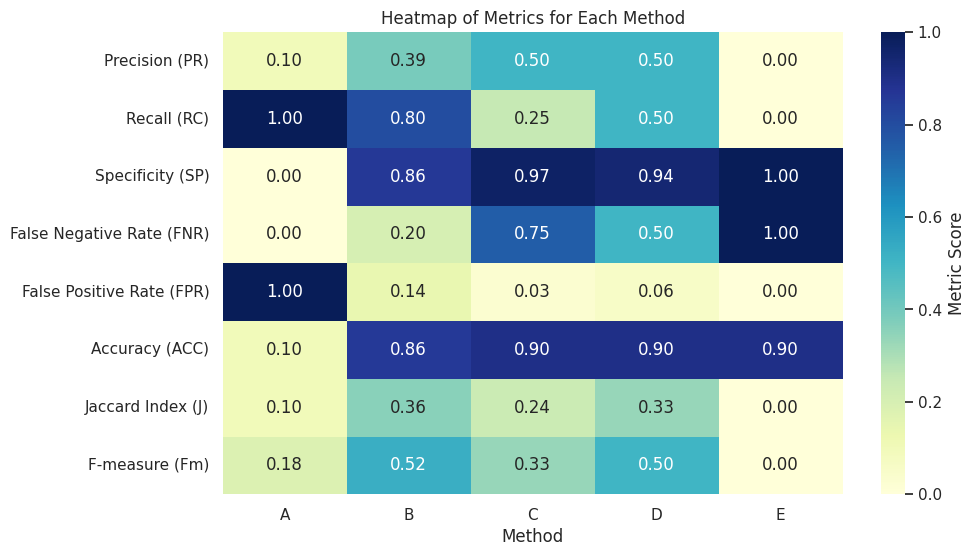
\includegraphics[width=.7\textwidth]{images/heatmap.png}
	\caption{Heatmap for metrics for each method}
	\label{fig:heatmap}
\end{figure}

To further clarify the performance of each method, we will introduce confusion matrices for each one. A confusion matrix offers a detailed view of the classification outcomes, highlighting the distribution of true positives, false positives, false negatives, and true negatives. Ideally, an optimal model will have a high number of true positives and true negatives while minimizing false positives and false negatives. In contrast, a poor-performing model will show high values for false positives and/or false negatives, indicating ineffective classification. Below, we present the confusion matrices for each method to visually compare their performances.

\begin{figure}[H]
	\centering
	\subfloat[Method A]{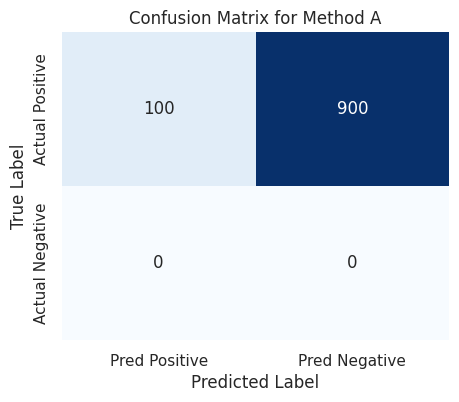
\includegraphics[width=0.3\textwidth]{images/confusion_matrixA}}
	\hspace{1em}
	\subfloat[Method B]{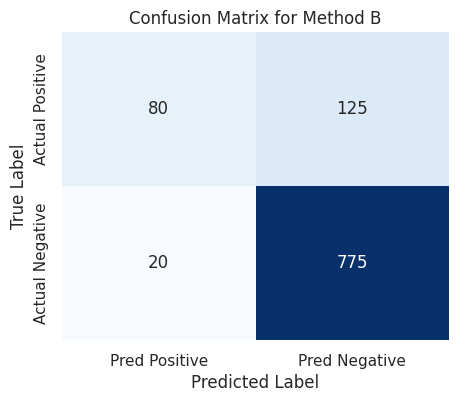
\includegraphics[width=0.3\textwidth]{images/confusion_matrixB}}
	\\
	\subfloat[Method C]{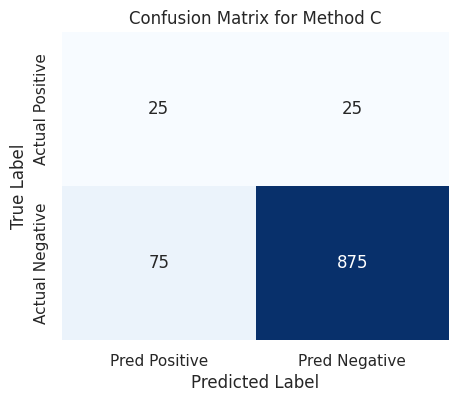
\includegraphics[width=0.3\textwidth]{images/confusion_matrixC}}
	\hspace{1em}
	\subfloat[Method D]{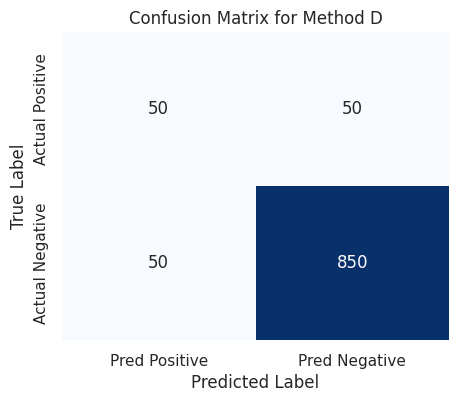
\includegraphics[width=0.3\textwidth]{images/confusion_matrixD}}
	\hspace{1em}
	\subfloat[Method E]{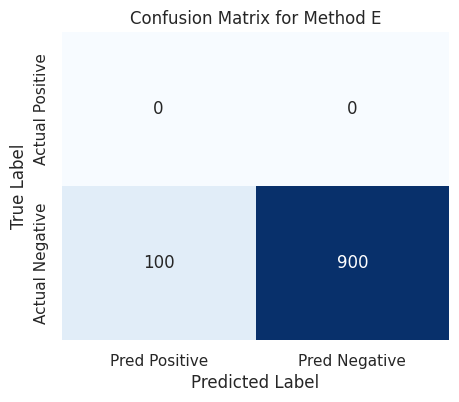
\includegraphics[width=0.3\textwidth]{images/confusion_matrixE}}
	\caption{Confusion matrices for each classification method.}
	\label{fig:confusion_matrices}
\end{figure}

\subsection{Performance Analysis}

For each metric, the following analysis highlights the best and worst methods, with a brief explanation for each:

\begin{itemize}
	\item \textbf{Precision (PR):} \\
	The best methods in terms of precision are Methods C and D (0.5000), showing that 50\% of their positive predictions are correct. This is beneficial for scenarios where accurate positive identification is key. Method E, however, scores the lowest (0.0), as it makes no positive predictions.
	
	\item \textbf{Recall (RC):} \\
	Method A achieves the highest recall (1.0000), identifying all actual positives correctly, which is ideal in cases where detecting all positives is essential, but in this case does not mean anything since the model only classifies as positive. Method E performs the worst (0.0), as it fails to classify any positives. 
	
	\item \textbf{Specificity (SP):} \\
	Method E has the highest specificity (1.0000), correctly classifying all negatives without any false positives. This is useful for minimizing false alarms. Method A, by contrast, has the lowest specificity (0.0), as it incorrectly classifies all negatives as positives. This is because method E classifies everithing as false and method A as true, which is a extremely bad classification.
	
	\item \textbf{False Negative Rate (FNR):} \\
	Method A has the lowest FNR (0.0), indicating it captures all positives without missing any. In contrast, Method E has the highest FNR (1.0), as it misses all positive cases, leading to poor detection of positives.
	
	\item \textbf{False Positive Rate (FPR):} \\
	The lowest FPR is achieved by Method E (0.0), as it avoids misclassifying any negatives as positives. Method A has the highest FPR (1.0) because it classifies all negatives as positives, resulting in many false positives.
	
	\item \textbf{Accuracy (ACC):} \\
	Methods C, D, and E exhibit the highest accuracy (0.9000), showing an effective balance between correctly identifying positives and negatives. Method A, with an accuracy of 0.1, performs the worst, as it misclassifies almost all negative instances.
	
	\item \textbf{Jaccard Index (J):} \\
	Method B achieves the highest Jaccard Index (0.3556), indicating a favorable overlap between predicted and actual positives. Method E, however, scores 0.0 on this metric due to its lack of positive predictions.
	
	\item \textbf{F-measure (Fm):} \\
	The highest F-measure is obtained by Method B (0.5246), showing a solid balance between precision and recall. Method E, again, scores the lowest (0.0), as it fails to identify any positives.
\end{itemize}

\begin{figure}[H]
	\centering
	\begin{minipage}{0.37\textwidth}
		\centering
		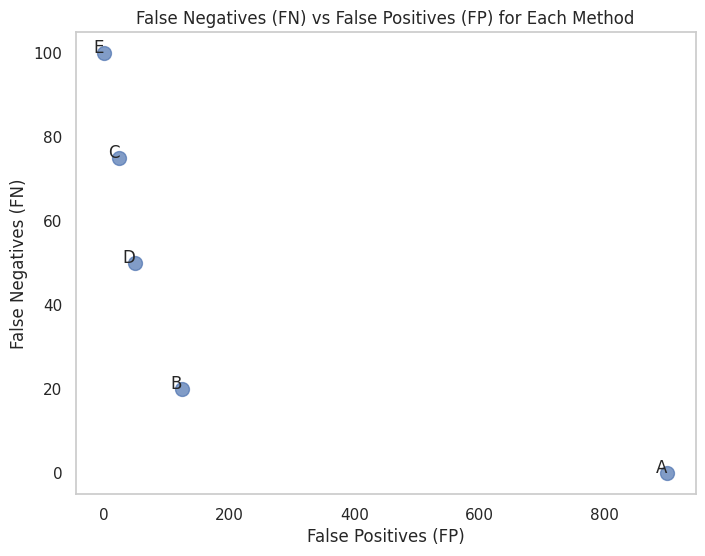
\includegraphics[width=\textwidth]{images/FN-FP.png}
		\caption{False Negatives VS False Positives}
		\label{fig:FN-FP}
	\end{minipage}
	\hspace{0.03\textwidth} % Espacio entre imágenes
	\begin{minipage}{0.37\textwidth}
		\centering
		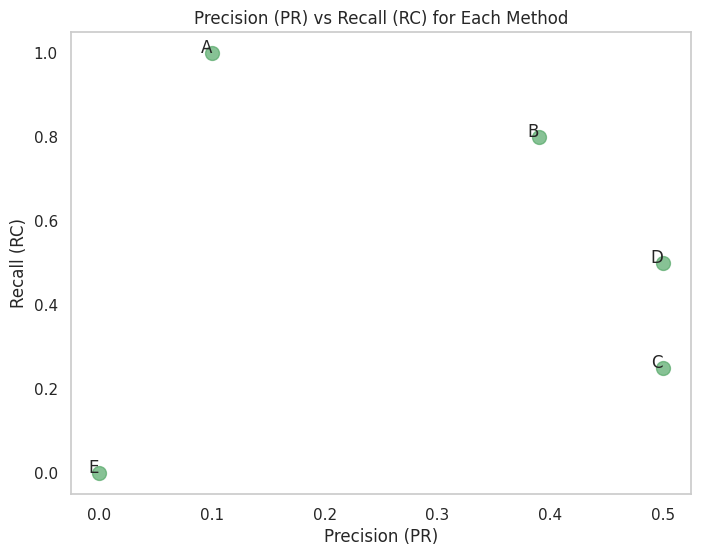
\includegraphics[width=\textwidth]{images/PR-RC.png}
		\caption{Precision VS Recall}
		\label{fig:PR-RC}
	\end{minipage}
	\hspace{0.03\textwidth} % Espacio entre imágenes
	\begin{minipage}{0.37\textwidth}
		\centering
		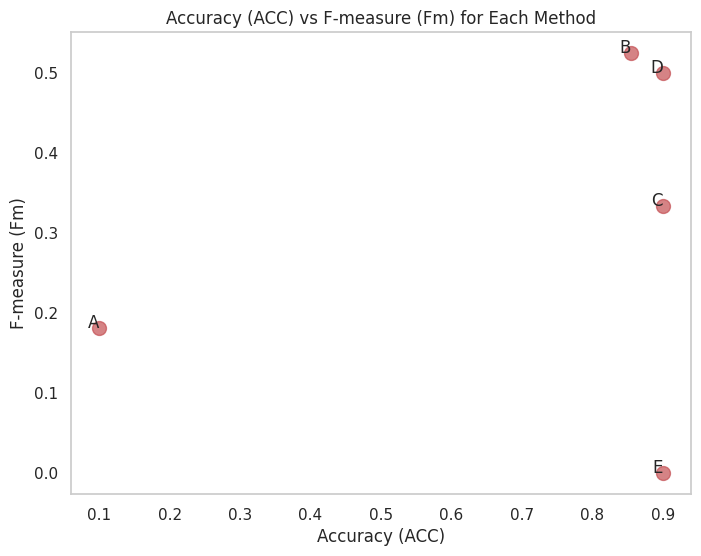
\includegraphics[width=\textwidth]{images/ACC-Fm.png}
		\caption{Accuracy VS F-measure}
		\label{fig:ACC-Fm}
	\end{minipage}
	
	\caption{Comparison of methods}
	\label{fig:comparison}
\end{figure}


The FN vs FP plot (\ref{fig:FN-FP}) shows that Method A, with the highest false positives and zero false negatives, favors capturing all positives but at the cost of many false positives. In contrast, Method E has no false positives but misses all positives, resulting in high false negatives. Methods C and D provide a better balance, with lower and relatively similar counts of false positives and false negatives. Among these, Method B appears to offer the best trade-off between reducing both error types.
\\

In the plot \ref{fig:PR-RC} that shows PR vs RC, Method A achieves high recall with very low precision, while Method E has both values at zero, reflecting its negative-only classification. Method B shows the best balance, with high recall and moderate precision, making it favorable in cases needing high recall. Methods C and D each have a precision of 0.5, but Method D achieves a more balanced performance overall, with equal precision and recall scores.
\\

The ACC vs Fm comparison in plot \ref{fig:ACC-Fm} shows that Methods C, D, and E achieve high accuracy, though only Method D balances this with a strong F-measure. Method B achieves the highest F-measure, indicating good precision and recall, though its accuracy is slightly lower than the others. Method A, with the lowest accuracy and F-measure, is less effective overall.
\\

To gain a more comprehensive view of each method's strengths and weaknesses, we included a radar plot of all metrics, offering an at-a-glance comparison. This visual highlights the varying performance across precision, recall, specificity, accuracy, false positive rate, and other metrics, making it easier to observe each method’s unique performance profile.
\\

\begin{figure}[H]
	
	\centering
	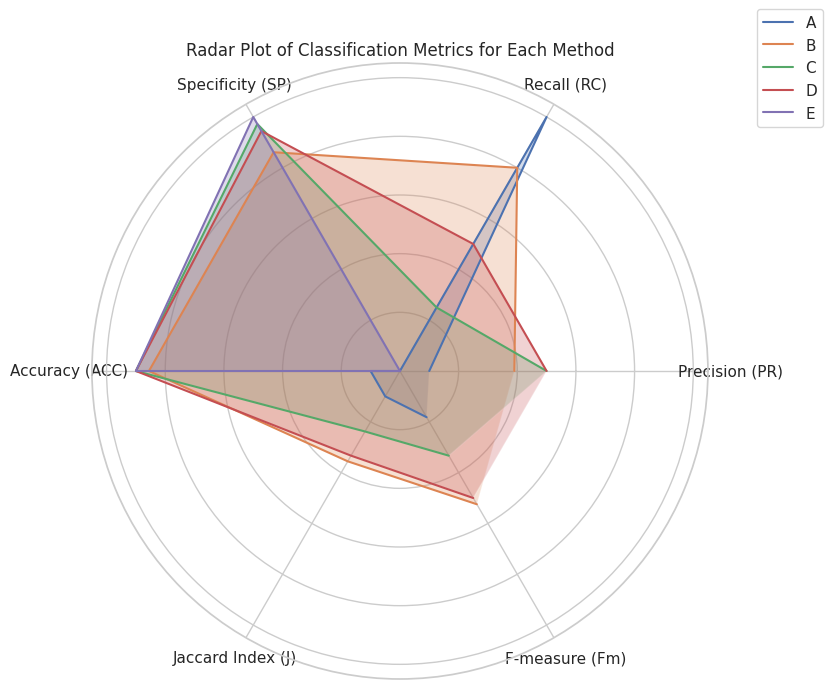
\includegraphics[width=.7\textwidth]{images/radar.png}
	\caption{Radar Plot of Classification Metrics}
	\label{fig:radar}
\end{figure}

In the radar plot \ref{fig:radar}, Method A stands out with its perfect recall but shows a sharp decline in precision, specificity, and accuracy, reinforcing its strategy of capturing all positives while sacrificing specificity and precision. Method B covers a broader area across most metrics, achieving high recall and moderate values in other metrics, making it the most balanced performer. Methods C and D show comparable profiles, though Method D consistently performs better in balancing precision, recall, and specificity, suggesting it as the most well-rounded choice among the high-accuracy methods. Method E has strong specificity but low values across most other metrics, aligning with its purely negative classification strategy.
\\

Overall, the radar plot offers a clear summary of each method’s performance, visually confirming that Method B provides the most balanced approach, while Method D remains the best choice for cases needing both high accuracy and strong class balance across metrics.
\\



\section{Conclusion}
In this study, we compared five classification methods (A, B, C, D, and E) based on a set of performance metrics to determine their effectiveness in handling an imbalanced dataset, particularly in the context of disease prediction. The results indicate varying levels of performance across precision, recall, and F-measure, with Method B emerging as the most balanced.

\begin{itemize}
	\item \textbf{Method B}: This method demonstrates the best overall balance across precision, recall, and F-measure, making it the most robust choice for applications that require both accurate positive identification and high precision.
	
	\item \textbf{Methods A and E}: These methods lack any meaningful classification capability. Method A only predicts positives and Method E only negatives, rendering both approaches ineffective for distinguishing between classes. Their limited functionality provides no valuable insight or accuracy for balanced classification tasks.
	
	\item \textbf{Method C}: This method achieves some balance between precision and specificity, yet it lacks the robustness of Method B due to an excessively high false negative rate.
	
	\item \textbf{Method D}: Although this method ranks as the second best, it has a higher false negative rate compared to Method B, which limits its overall effectiveness.
\end{itemize}



In summary, Method B is the most effective classification method for this dataset based on its high F-measure, balanced precision, and recall. This approach is recommended for predictive tasks where both the accurate identification of positives and the minimization of false positives are essential, even within an imbalanced dataset context.


\section{Repository Access}

All additional information, including the source code and full documentation of this project, is available in the GitHub repository \cite{cuevas2024github}.


% Incluir la bibliografía
\bibliographystyle{plain}  % Estilo de la bibliografía (por ejemplo, plain, alpha, ieee, etc.)
\bibliography{bibli}  % Nombre del archivo .bib sin la extensión

\end{document}
